% =====================================================================
%  Introductory poster — A0 portrait (841 x 1189 mm  =  33.1 x 46.8 in)
%  Built from presentation_structured_experiments.tex
%  Scope: problem + dataset + experiment design.  NO results.
% =====================================================================
\documentclass[25pt, a0paper, portrait, margin=18mm, innermargin=18mm,
               blockverticalspace=16mm, colspace=18mm, subcolspace=10mm]{tikzposter}

\usepackage{amsmath, amssymb, booktabs, array, graphicx}
\usepackage{tikz}
\usetikzlibrary{positioning, shapes.geometric, arrows.meta, fit, backgrounds, matrix, calc}

% ---- Palette (matches the talk's green/orange accents) --------------
\definecolor{accent}{HTML}{2E7D52}     % green
\definecolor{accentd}{HTML}{1B5E3A}
\definecolor{envcol}{HTML}{C77A0A}     % orange (environment)
\definecolor{paper}{HTML}{FBFBF8}
\definecolor{blocktitlebg}{HTML}{EAF3EC}

% ---- Theme ----------------------------------------------------------
\usetheme{Default}
\usecolorstyle{Germany}
\colorlet{backgroundcolor}{paper}
\colorlet{framecolor}{accentd}
\colorlet{titlefgcolor}{white}
\colorlet{titlebgcolor}{accentd}
\colorlet{blocktitlebgcolor}{blocktitlebg}
\colorlet{blocktitlefgcolor}{accentd}
\colorlet{notebgcolor}{envcol!18}
\colorlet{notefrcolor}{envcol}

\settitle{
  \centering
  \vbox{
    \color{titlefgcolor}
    {\Huge\bfseries Predicting Psychiatric Illness Risk from\\[6pt]
      Neuroimaging--Genetics Associations\par}
    \vspace{14pt}
    {\LARGE Leon Ackermann \quad\textbullet\quad Master Thesis \par}
    \vspace{8pt}
    {\large Using SNP associations to brain structure as an intermediate to predict psychiatric disease risk}
  }
}

% reusable node styles for the causal graph
\tikzset{
  cnode/.style={draw, rounded corners, fill=accent!14, draw=accent!75!black,
                line width=1.2pt, minimum width=4.6cm, minimum height=2.4cm,
                align=center, font=\Large\bfseries},
  envnode/.style={draw, rounded corners, fill=envcol!16, draw=envcol!80!black,
                  line width=1.2pt, minimum width=5.2cm, minimum height=2.2cm,
                  align=center, font=\Large\bfseries},
  carr/.style={-{Latex[length=6mm]}, line width=2pt},
}

\begin{document}
\maketitle

% =====================================================================
%  ROW 1 — THE PROBLEM
% =====================================================================
\begin{columns}
\column{0.5}
\block{The problem}{
  \large
  \textbf{Psychiatric disorders are highly polygenic.}
  Hundreds to thousands of common variants (SNPs) each contribute a tiny
  effect --- there is no single ``disease gene''. This makes risk hard to
  predict directly from genetics.

  \vspace{8pt}
  \textbf{Our idea.} A SNP may act on illness \emph{through brain structure}.
  We therefore use a SNP's measured associations to $\sim$1{,}000
  MRI-derived brain phenotypes as features, and ask whether they predict that
  SNP's association to the illness.

  \vspace{8pt}
  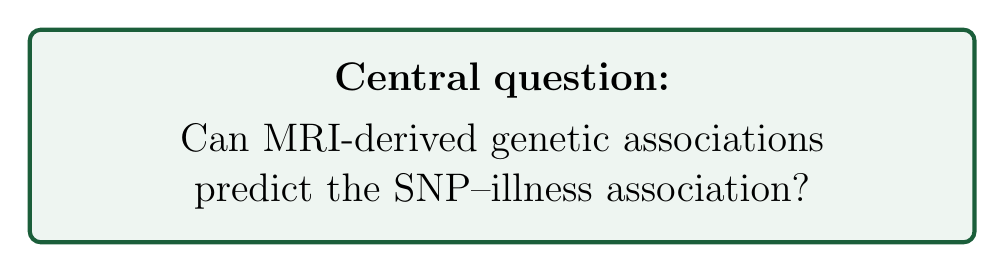
\begin{tikzpicture}
    \node[draw=accentd, line width=1.5pt, rounded corners, fill=accent!8,
          inner sep=12pt, text width=0.92\linewidth, align=center, font=\Large] {
      \textbf{Central question:}\\[4pt]
      Can MRI-derived genetic associations predict the SNP--illness association?
    };
  \end{tikzpicture}
}

\column{0.5}
\block{What we hope to gain}{
  \large
  \begin{itemize}\setlength\itemsep{8pt}
    \item Identify \textbf{neurobiological biomarkers} --- the specific brain
          regions / phenotypes that carry illness signal.
    \item Test whether the MRI$\,\to\,$illness link is \textbf{non-linear}
          rather than purely linear.
    \item Build a \textbf{structured pathway} from genetics to disease, rather
          than a black-box genotype$\to$phenotype predictor.
  \end{itemize}
  \vspace{6pt}
  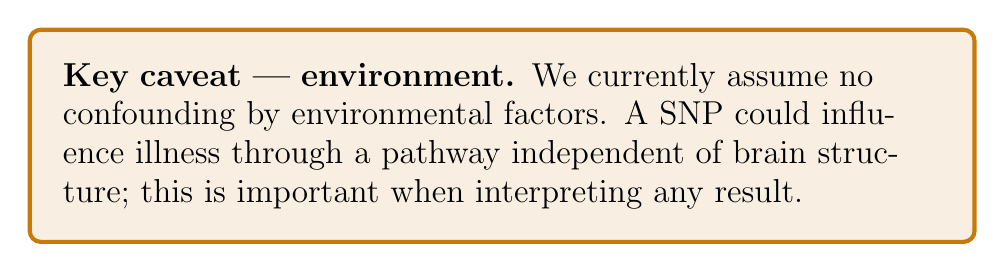
\begin{tikzpicture}
    \node[draw=envcol, line width=1.5pt, rounded corners, fill=envcol!12,
          inner sep=12pt, text width=0.92\linewidth, align=left, font=\large] {
      \textbf{Key caveat --- environment.} We currently assume no
      confounding by environmental factors. A SNP could influence illness through
      a pathway independent of brain structure; this is important when
      interpreting any result.};
  \end{tikzpicture}
}
\end{columns}

% =====================================================================
%  ROW 2 — HERO CAUSAL GRAPH  (SNP / MRI / Illness / Environment)
%          with the candidate "networks" on the prediction arrow
% =====================================================================
\block{From genetics to illness through the brain --- and the models that learn the link}{
\centering
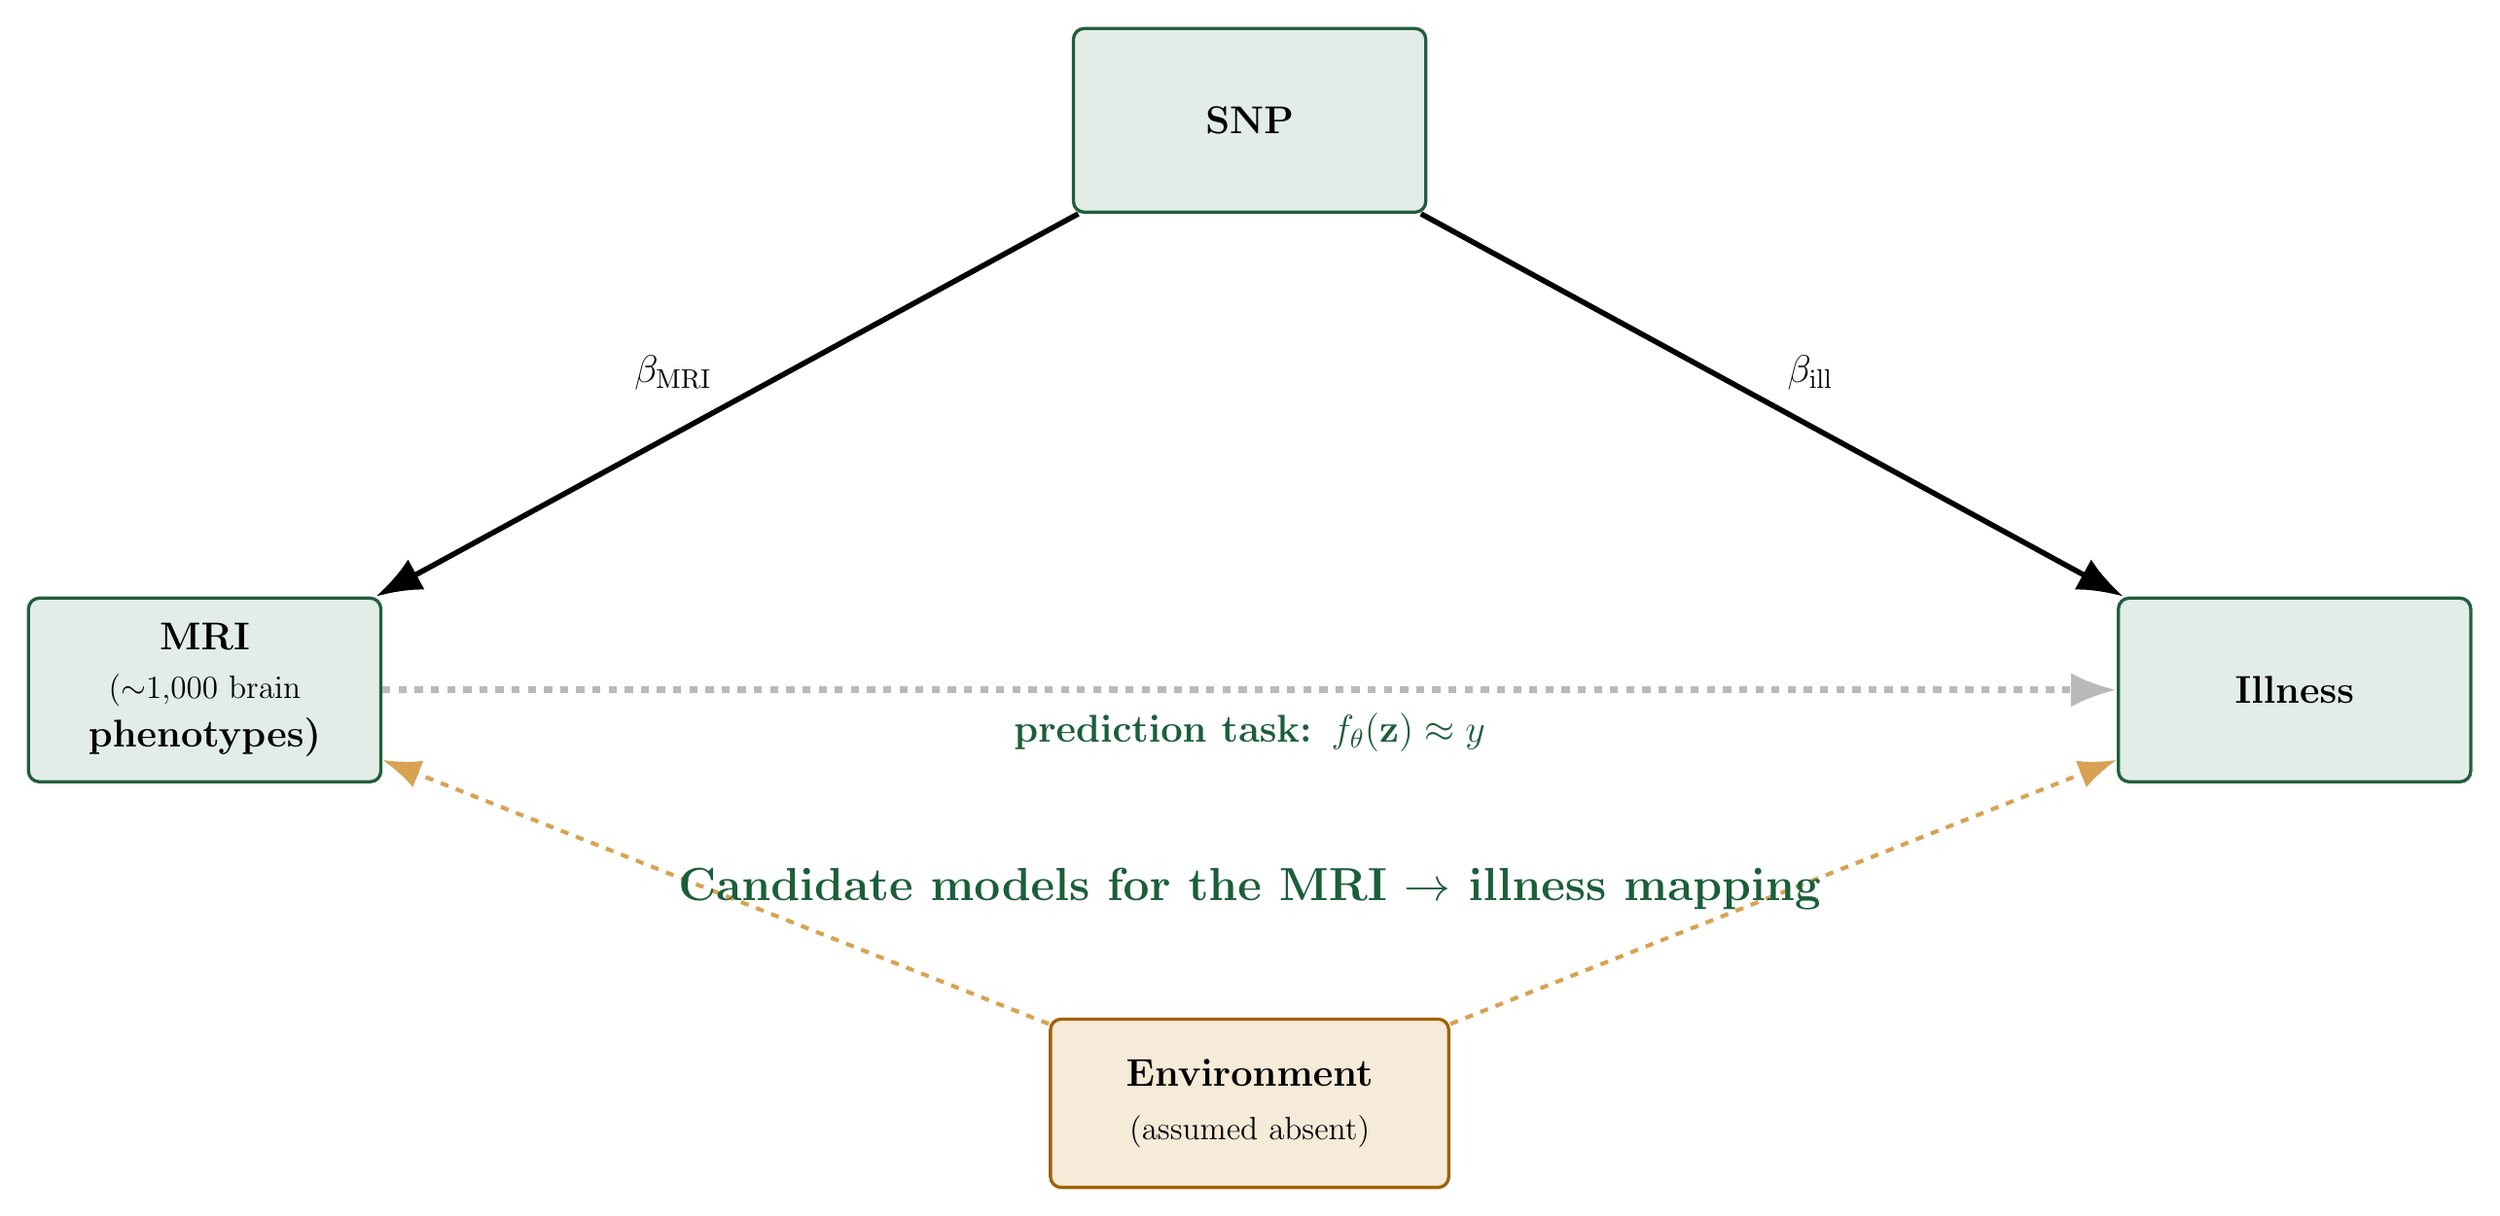
\begin{tikzpicture}[node distance=4.5cm and 7cm]

  % --- causal DAG ---------------------------------------------------
  \node[cnode] (snp) {SNP};
  \node[cnode, below left=5cm and 9cm of snp]  (mri) {MRI\\\large\mdseries($\sim$1{,}000 brain\\ phenotypes)};
  \node[cnode, below right=5cm and 9cm of snp] (ill) {Illness};
  \node[envnode, below=10.5cm of snp] (env) {Environment\\[2pt]\large\mdseries(assumed absent)};

  \draw[carr] (snp) -- node[above left=2pt, font=\Large]{$\beta_{\mathrm{MRI}}$} (mri);
  \draw[carr] (snp) -- node[above right=2pt, font=\Large]{$\beta_{\mathrm{ill}}$} (ill);
  \draw[carr, dashed, gray!55, line width=2.5pt]
        (mri) -- node[below=4pt, font=\Large\bfseries, text=accentd]{prediction task: $f_\theta(\mathbf{z})\approx y$} (ill);

  % environment dashed influences (faded)
  \draw[-{Latex[length=5mm]}, dashed, envcol!70, line width=1.5pt] (env) -- (mri);
  \draw[-{Latex[length=5mm]}, dashed, envcol!70, line width=1.5pt] (env) -- (ill);

  % --- big arrow from the prediction link down to the model zoo -----
  \coordinate (mid) at ($(mri)!0.5!(ill)$);
  \node[below=2.2cm of mid, font=\LARGE\bfseries, text=accentd] (zoolab)
        {Candidate models for the MRI $\to$ illness mapping};

\end{tikzpicture}

\vspace{4pt}
% ---- the four candidate "networks" in a row -----------------------
\begin{tikzpicture}[
  mbox/.style={draw=accent!70!black, line width=1pt, rounded corners,
               fill=white, inner sep=12pt, minimum height=9cm, anchor=north},
  mcap/.style={font=\Large\bfseries, text=accentd, anchor=north}]

  % ---- (1) Linear / regularised regression -----------------------
  \node[mbox] (m1) at (0,0) {
    \begin{tikzpicture}[
      innode/.style={draw, circle, fill=blue!15, minimum size=0.9cm, inner sep=0pt, font=\small},
      outnode/.style={draw, circle, fill=orange!25, minimum size=1.1cm, inner sep=0pt, font=\small},
      arr/.style={->, gray!60!black}]
      \node[innode] (i1) at (0, 1.6) {$z_1$};
      \node[innode] (i2) at (0, 0.7) {$z_2$};
      \node          at (0,-0.1) {$\vdots$};
      \node[innode] (im) at (0,-1.0) {$z_m$};
      \node[outnode] (o) at (3,0.3) {$\hat y$};
      \draw[arr] (i1)--(o); \draw[arr] (i2)--(o); \draw[arr] (im)--(o);
      \node[font=\small] at (1.5,2.4) {$\hat y=\mathbf{w}^\top\mathbf{z}+b$};
    \end{tikzpicture}};

  % ---- (2) Gradient boosted trees --------------------------------
  \node[mbox, right=2.5cm of m1] (m2) {
    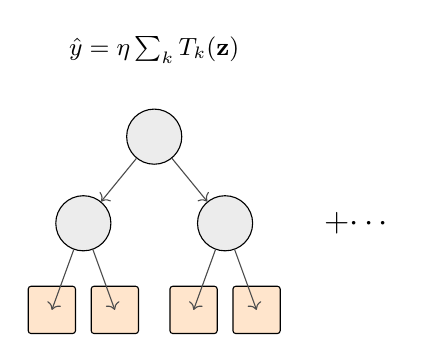
\begin{tikzpicture}[
      nd/.style={draw, circle, fill=gray!15, minimum size=0.7cm, inner sep=0pt},
      lf/.style={draw, fill=orange!20, rounded corners=1pt, minimum size=0.6cm, inner sep=1pt},
      arr/.style={->, gray!60!black}]
      \node[nd] (r) at (0,0.6) {}; \node[nd] (l) at (-0.9,-0.5) {}; \node[nd] (rr) at (0.9,-0.5) {};
      \node[lf] at (-1.3,-1.6){}; \node[lf] at (-0.5,-1.6){};
      \node[lf] at (0.5,-1.6){};  \node[lf] at (1.3,-1.6){};
      \draw[arr](r)--(l);\draw[arr](r)--(rr);
      \draw[arr](l)--(-1.3,-1.6);\draw[arr](l)--(-0.5,-1.6);
      \draw[arr](rr)--(0.5,-1.6);\draw[arr](rr)--(1.3,-1.6);
      \node[font=\large] at (2.6,-0.5) {$+\!\cdots$};
      \node[font=\small] at (0.0,1.7) {$\hat y=\eta\sum_k T_k(\mathbf{z})$};
    \end{tikzpicture}};

  % ---- (3) Regularised MLP (ResidualDNN) -------------------------
  \node[mbox, right=2.5cm of m2] (m3) {
    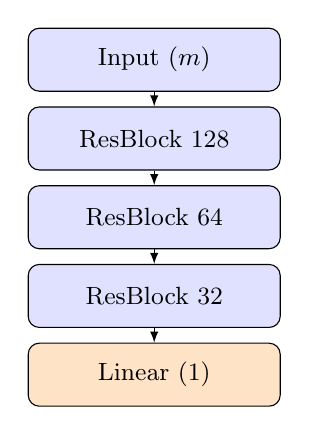
\begin{tikzpicture}[
      block/.style={draw, rounded corners, minimum width=3.2cm, minimum height=0.8cm, fill=blue!12, align=center, font=\small}]
      \node[block] (a) at (0,1.8)  {Input ($m$)};
      \node[block] (b) at (0,0.8)  {ResBlock 128};
      \node[block] (c) at (0,-0.2) {ResBlock 64};
      \node[block] (d) at (0,-1.2) {ResBlock 32};
      \node[block, fill=orange!22] (e) at (0,-2.2) {Linear (1)};
      \draw[-latex](a)--(b);\draw[-latex](b)--(c);\draw[-latex](c)--(d);\draw[-latex](d)--(e);
    \end{tikzpicture}};

  % ---- (4) TabPFNv2 ----------------------------------------------
  \node[mbox, right=2.5cm of m3] (m4) {
    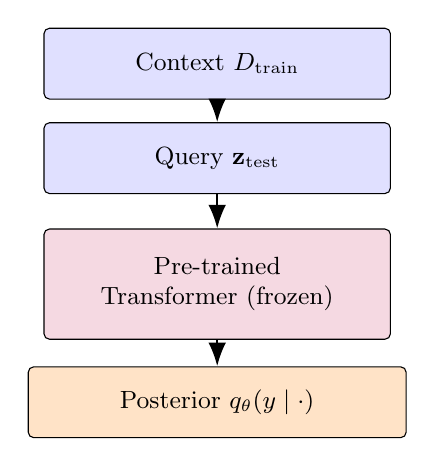
\begin{tikzpicture}[
      blk/.style={draw, rounded corners=2pt, minimum width=4.4cm, minimum height=0.9cm, fill=blue!12, align=center, font=\small},
      tfb/.style={draw, rounded corners=2pt, minimum width=4.4cm, minimum height=1.4cm, fill=purple!15, align=center, font=\small},
      outb/.style={draw, rounded corners=2pt, minimum width=4.8cm, minimum height=0.9cm, fill=orange!22, align=center, font=\small},
      arr/.style={-{Latex[length=3mm]}, thick}]
      \node[blk] (ctx) at (0,1.9)  {Context $D_{\text{train}}$};
      \node[blk] (qry) at (0,0.7)  {Query $\mathbf{z}_{\text{test}}$};
      \node[tfb] (tf)  at (0,-0.9) {Pre-trained\\Transformer (frozen)};
      \node[outb](ou)  at (0,-2.4) {Posterior $q_\theta(y\mid\cdot)$};
      \draw[arr](ctx)--(qry);\draw[arr](qry)--(tf);\draw[arr](tf)--(ou);
    \end{tikzpicture}};

  % ---- captions --------------------------------------------------
  \node[mcap] at ($(m1.south)+(0,-0.4)$) {Linear / Ridge / Lasso};
  \node[mcap] at ($(m2.south)+(0,-0.4)$) {XGBoost (trees)};
  \node[mcap] at ($(m3.south)+(0,-0.4)$) {ResidualDNN (MLP)};
  \node[mcap] at ($(m4.south)+(0,-0.4)$) {TabPFNv2 (in-context)};
\end{tikzpicture}

\vspace{6pt}
{\large Each model learns $f_\theta:\mathbb{R}^{m}\!\to\!\mathbb{R}$,
mapping a SNP's MRI z-score profile $\mathbf{z}$ to its illness z-score $y$,
fit by mean-squared-error empirical risk minimisation.}
}

% =====================================================================
%  ROW 3 — DATASET
% =====================================================================
\begin{columns}
\column{0.5}
\block{The dataset --- source GWAS}{
  \large
  Inputs are publicly available \textbf{GWAS summary statistics}. For SNP $i$
  and phenotype $j$ we use the z-score $z_{i,j}=\beta_{i,j}/\mathrm{s.e.}(\beta_{i,j})$.
  All cohorts are of European ancestry.

  \vspace{8pt}
  \centering\renewcommand{\arraystretch}{1.25}
  \begin{tabular}{@{}llrr@{}}
    \toprule
    \textbf{Phenotype} & \textbf{Consortium} & \textbf{$N_{\text{case}}$} & \textbf{$N_{\text{control}}$}\\
    \midrule
    \multicolumn{4}{@{}l}{\emph{MRI: $\approx$1{,}000 brain features (UK Biobank)}}\\
    \midrule
    SCZ  & PGC-SWG    & 53{,}386 & 77{,}258\\
    BIP  & PGC        & 59{,}287 & 781{,}022\\
    MDD  & PGC-MDD    & 59{,}851 & 113{,}154\\
    ADHD & PGC-iPSYCH & 38{,}691 & 186{,}843\\
    AZ   & IGAP-UKB   & 71{,}880 & 383{,}378\\
    OCD  & PGC-OCD    & 23{,}493 & 1{,}114{,}613\\
    \bottomrule
  \end{tabular}

  \vspace{8pt}
  \large \textbf{SCZ} has the largest GWAS $\Rightarrow$ strongest signal, and
  is our primary testbed.
}

\column{0.5}
\block{Construction pipeline (per illness)}{
  \centering
  \includegraphics[width=0.98\linewidth]{../presentation/figures/pipeline.png}

  \vspace{6pt}
  \raggedright\large
  \textbf{Steps:} harmonise alleles across cohorts $\rightarrow$
  \textbf{LD-clump} ($R^2<0.05$) to keep independent SNPs $\rightarrow$
  merge MRI and illness GWAS on shared lead SNPs.

  \vspace{10pt}
  \textbf{Result: one tabular dataset per illness.}
  Rows $=$ SNPs, features $=$ MRI z-scores, target $=$ illness z-score:
  \vspace{4pt}
  \[
  \left[\;
  \begin{array}{cccc|c}
  z_{1,1} & z_{1,2} & \cdots & z_{1,m} & y_{1}\\
  z_{2,1} & z_{2,2} & \cdots & z_{2,m} & y_{2}\\
  \vdots  & \vdots  & \ddots & \vdots  & \vdots\\
  z_{N,1} & z_{N,2} & \cdots & z_{N,m} & y_{N}
  \end{array}
  \;\right]\quad m\approx 1{,}000
  \]
}
\end{columns}

% =====================================================================
%  ROW 4 — EXPERIMENT DESIGN (few words)
% =====================================================================
\block{Experiment design --- a 2$\times$2 grid over the causal graph}{
\large
The SNP is the common cause; each arrow carries its own GWAS $p$-value. Two
filters --- on the \textbf{MRI} arrow and on the \textbf{illness} arrow ---
cross into four datasets, each isolating a different signal/noise mix.
\vspace{10pt}

\centering
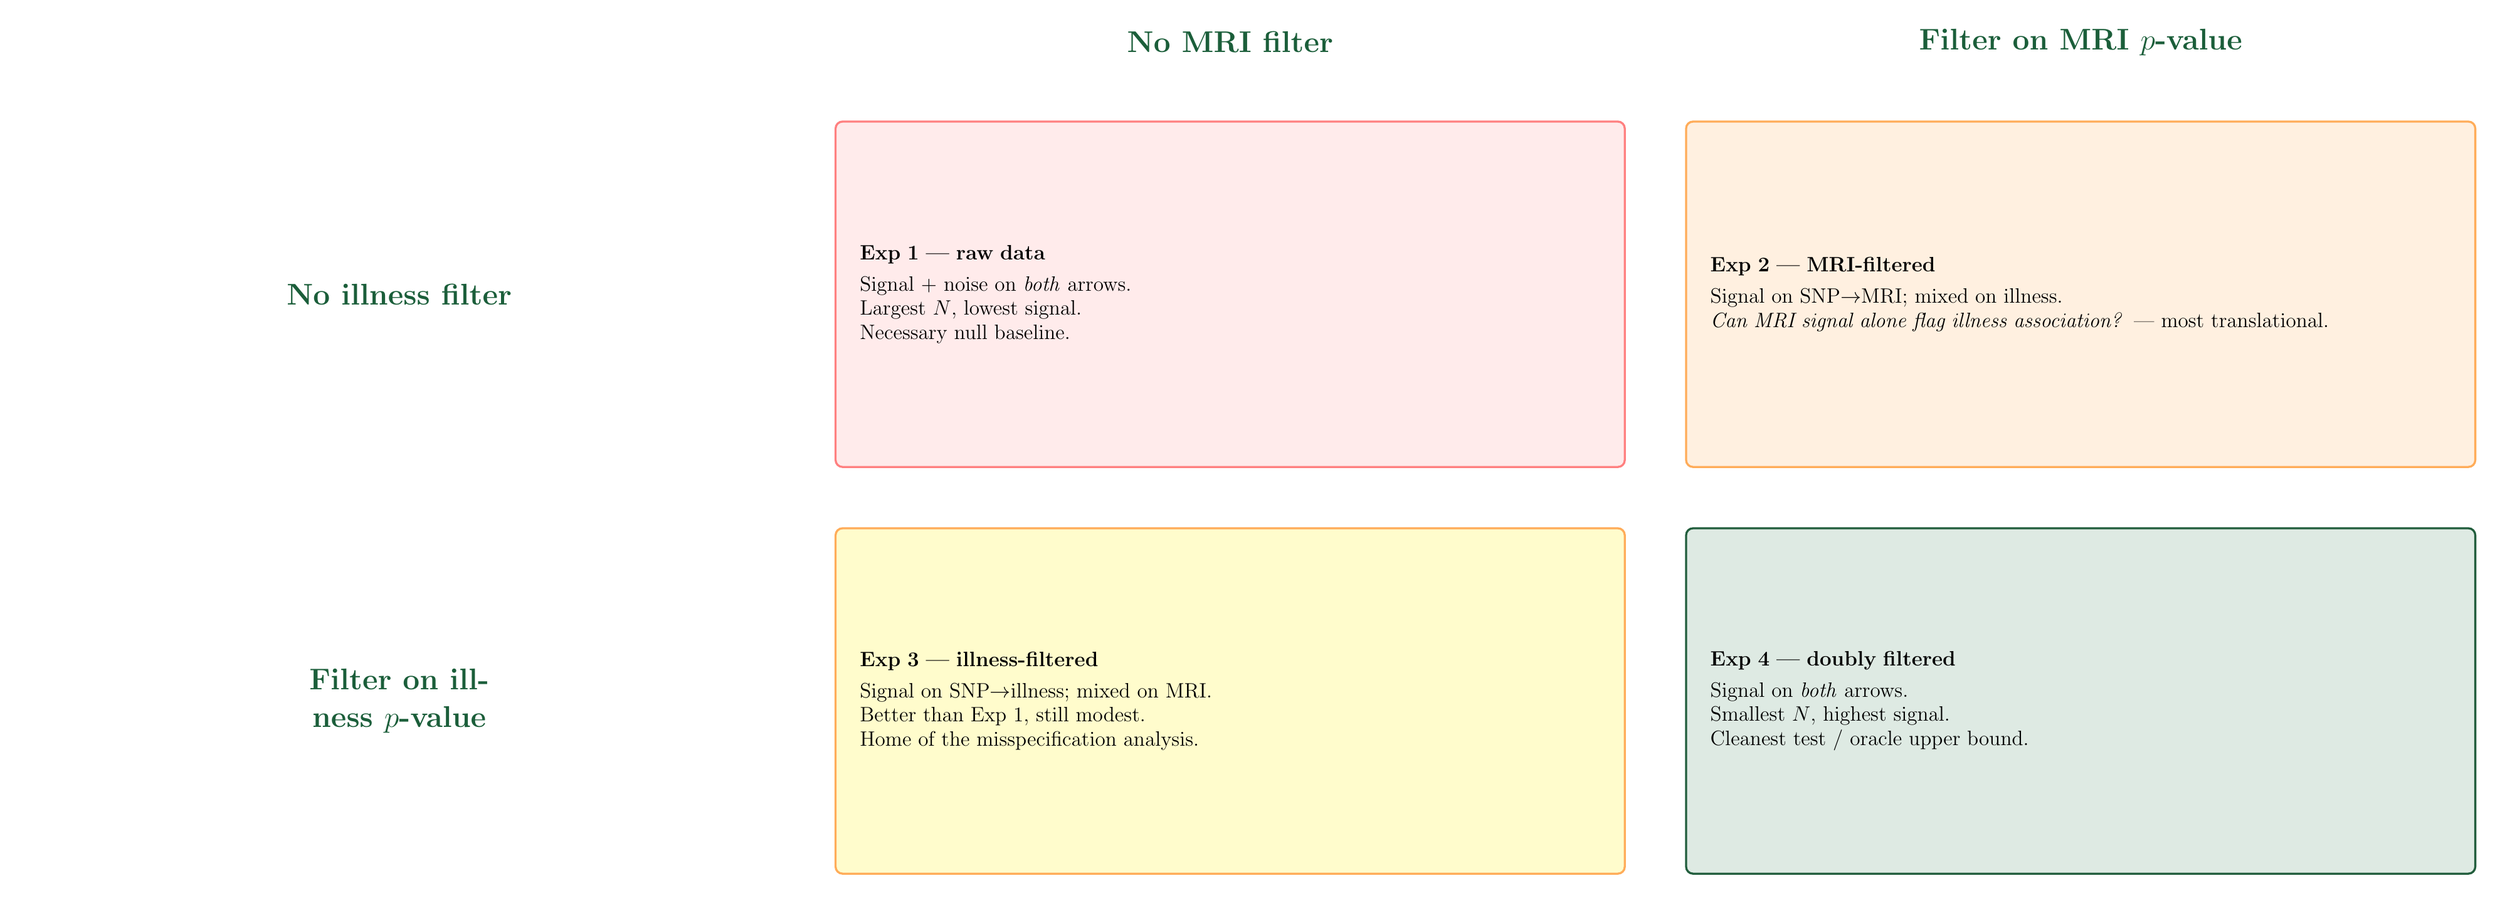
\begin{tikzpicture}[
  every node/.style={font=\large},
  cell/.style={draw, rounded corners=4pt, text width=15cm, minimum height=7cm,
               align=left, inner sep=14pt, anchor=center, line width=1.2pt},
  e1/.style={cell, fill=red!8,     draw=red!50},
  e2/.style={cell, fill=orange!12, draw=orange!65},
  e3/.style={cell, fill=yellow!20, draw=orange!65},
  e4/.style={cell, fill=accent!16, draw=accent!75!black},
  colhdr/.style={font=\LARGE\bfseries, anchor=center, text width=15cm, align=center, text=accentd},
  rowhdr/.style={font=\LARGE\bfseries, anchor=center, align=center, text width=6cm, text=accentd}]

\matrix (G) [matrix of nodes, nodes in empty cells,
    column sep=1.2cm, row sep=1.2cm,
    column 1/.style={nodes={rowhdr}}, row 1/.style={nodes={colhdr}},
    ampersand replacement=\&]{
        \& No MRI filter \& Filter on MRI $p$-value \\
  {No illness filter}
        \& |[e1]|{\textbf{Exp 1 --- raw data}\\[4pt]
                  Signal + noise on \emph{both} arrows.\\
                  Largest $N$, lowest signal.\\
                  Necessary null baseline.}
        \& |[e2]|{\textbf{Exp 2 --- MRI-filtered}\\[4pt]
                  Signal on SNP$\to$MRI; mixed on illness.\\
                  \emph{Can MRI signal alone flag illness
                  association?} --- most translational.} \\
  {Filter on illness $p$-value}
        \& |[e3]|{\textbf{Exp 3 --- illness-filtered}\\[4pt]
                  Signal on SNP$\to$illness; mixed on MRI.\\
                  Better than Exp 1, still modest.\\
                  Home of the misspecification analysis.}
        \& |[e4]|{\textbf{Exp 4 --- doubly filtered}\\[4pt]
                  Signal on \emph{both} arrows.\\
                  Smallest $N$, highest signal.\\
                  Cleanest test / oracle upper bound.} \\
};
\end{tikzpicture}

\vspace{10pt}
\large
\textbf{Protocol.} Same four model families in every cell; 80/20 train/test
split, 5 seeds, nested cross-validation for hyperparameters (Optuna).
Metrics: $R^2$ and squared correlation. \emph{Reading the cells pairwise
isolates the marginal contribution of each filter.}
}

\end{document}
